\section{Example of applications for Monte Carlo simulations}
\label{sec:examples}
\subsection{Emulation of electromagnetic interaction models}
\subsection{Emulation of low energy nuclear interaction models}
\subsection{Emulation of radiation-matter interactions}
\label{subsec:interactions}
%tommaso
% computational cost of full fledged simulations; their not complete ability to match data

DOES THIS GO TO THE INITIAL PART OF THE SECTION???
One of the most complex tasks in Monte Carlo simulations involving the use of detectors (medical apparatuses, particle physics detectors) lies in the dual need of being able to optimize the design before detector construction, and to simulate the behavior under working conditions after the setup has been prepared.
In both cases, unless the setup is very similar to existing detectors, extensive Monte Carlo simulations of the expected detector capabilities are the widely used solutions. Various such tools exist (Geant4\cite{g4}, Fluka\cite{fluka}, MCNPX\cite{MCNPX}), with different application regimes and specific utilization patterns. As a general rule, these implement iteratively basic radiation-matter low-level processes to a knowledge of the detector setup, including materials, geometry and  XXX; as such, they incur into two general limits:
\begin{itemize}
\item a scarce capability to be tuned to experimental results, by changing the basic modelling of the processes;
\item a large to very large need for computational resources, given the iteration oriented approach and the need to increase the level of iterations in order to obtain a better precision and adherence to data.
\end{itemize}

% Geant4, Fluka, MCNPX: https://doi.org/10.1063/1.2720459

Both limitations can in principle be surpassed via the use of Artificial Intelligence oriented tools.
In presence of experimental data, the response of the AI system can be tuned to that without any explicit modelling of the physics processes; speed can be vastly improved by the change from iterative-based computations to standard Deep Learning matrix algebra, with intrinsic capabilities for high performance processing on, for example, GPU systems.

As an example we want to consider here CaloGan\cite{calogan}, an attempt to reproduce the details of radiation-matter interactions in the complex setup of segmented (3 layers) electromagnetic calorimeters.
A generative Adversarial Network, as those presented in Section~\ref{subsec:gan}, is used in conjunction with an as much-as-accurate as possible Geant4 simulation of the detector setup. The generator side accepts in input input particle 4-momentum, ad after the passage through quite standard convolutional (matching the detector response as 2-D images) and dense layers, the output is compared with Geant4 simulations of a particle with the same parameters.  The training optimizes the energy deposition per layer and per 2-D transverse cell, in a way in principle suited also for using real data in input. Results are very encouraging, even in a detector scenario which can be considered as extreme: not only the quantities of direct training are well reproduced, but also secondary and derived quantities like shower shapes are in most cases well described.

ADD DISCUSSION and PLOT



A second similar attempt, applied to the not-yet existing CLIC proposed electromagnetic and hadronic calorimeter, is presented in~\cite{3dgan}, with the goal to directly reproduce 3-D signals in a high granular calorimeter. The reference dataset, in absence of real data, is has the form of Geant4 generated showers sampled in a 25x25x25 cells around the impinging particle.
% https://doi.org/10.1051/epjconf/201921402010
Figure~\ref{fig:3dgan_shower_longitudinal} shows the longitudinal shower shapes for 100 GeV electrons in the electromagnetic part of the calorimeter compared with detailed Geant4 simulations. The level of agreement is very satisfactory.

In sections~\ref{subsec:speed} and ~\ref{subsec:physical} we will discuss about the speed gain with respect to standard methods, and solutions and needs to prevent unphysical results.

\subsection{Emulation of detector responses}
Monte Carlo tools like Geant4 are designed to simulate, as accurately as possible, the energy deposition (in keV, for example) happening because of the passage on particle / radiation in the material of a detector. In real life, what a scientist measures is instead the response, in forms of analog or digital signals, of a measuring device in which energy deposition is read and processed by some electronics. Hence, in classical systems, the simulation of radiation / matter must be followed by an ad-hoc simulation of the electronic readout system, in order to be compared with actual readings from a detector. In the case of AI inspired tools, this can be avoided by completely bypassing the "energy deposition" output results, and training the system directly with real or realistic (from the above ad-hoc simulation) signals from the electronic back-end. In ~\cite{mri}, for example, images from a real MRI apparatus are used for the training the system (see Figure~\ref{fig:elec}); the use of more classical approaches would be indeed more problematic since there is no practical way to measure (and validate) the output in terms of energy deposition in a running system.
\begin{figure}[h]
    \centering

    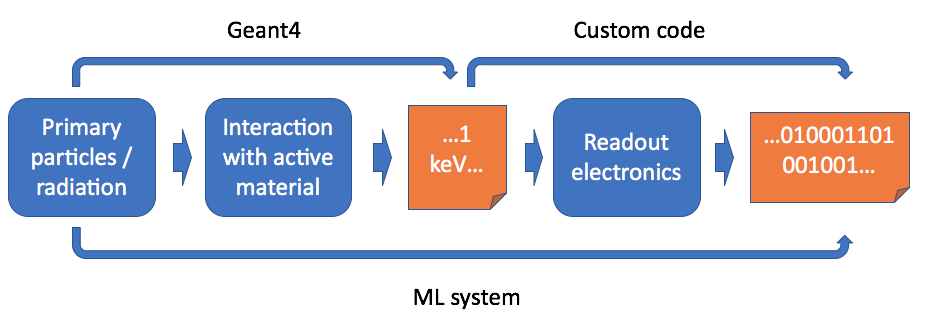
\includegraphics[width=0.8\textwidth]{images/electronics.png}
    \caption{Difference between classical and AI inspired simulation of experimental setups.}
     \label{fig:elec}

\end{figure}

%ale: trovi tu una referenza decente questo
%tommaso
